\chapter{Teoretická část}\label{chap:teorie}


\section{Virtualizace}

Koncept virtualizace se poprvé objevil na konci 50.\,let minulého století, kdy skupina z University v Manchesteru vytvořila první funkční prototyp virtuální paměti. Následně v 60.\, letech minulého století byl koncept rozšířen i na celé počítače. První tzv. \textit{virtual machine} (VM), neboli česky \uv{virtuální stroj}, byl vytvořen firmou IBM a jejich cílem bylo umožnit souběžný přístup k sálovým počítačům. Každá VM byla instancí fyzického stroje a dávala iluzi toho, že uživatel přistupuje přímo k fyzickému stroji. Uživatelé mohli vyvíjet, spouštět a testovat aplikace bez obavy toho, že by mohli zhroutit celý počítač, díky tomu, že každá VM byla izolovaná kopie systému. 

Polovinou 70.\,let minulého století byla virtualizace dobře akceptovaným konceptem mezi uživateli. Použitím virtualizace totiž mohli vyřešit podstatné problémy této doby. Například díky již zmíněné virtualizované paměti mohli uživatelé adresovat mnohem větší operační paměť, než počítač skutečně obsahoval. 

Všechny tyto virtualizační techniky byly primárně cesta k vyrovnání se s vysokou pořizovací cenou hardwaru v této době. Díky ní mohli majitelé sálových počítačů využít svoji investici co nejefektivněji. Její použití se tedy se snižujícími cenami hardwaru začalo snižovat a dokonce skoro vymizelo během 80. a 90.\,let díky příchodu levnějších osobních počítačů.  

Poptávka po virtualizaci začala znovu růst až v 90.\,letech minulého století. Se zvětšující se různorodostí hardwaru a softwaru zde vznikla poptávka na to, aby bylo možné spustit aplikace, které původně byly určeny pro jiný hardware a jiný operační systém, na jednom určitém stroji. Poptávka se ovšem zvětšila i v komerčním sektoru. Se zvyšujícími počty serverů firmy hledaly způsoby, jak využít investici do serveru naplno. Spustit pouze jednu aplikaci na serveru nebylo příliš ekonomické, jelikož tato aplikace nemusela vždy využít všechny výpočetní zdroje, a nákup dalších serverů přinášel mimo samotné pořizovací ceny i další náklady, například na údržbu. Řešení pro tento problém tedy byla opět virtualizace. Oba tyto trendy pokračují do dnes a jsou jedny z hlavních důvodů pro použití virtualizace. 

Virtualita se od reality liší pouze ve formálním světě. Má ovšem podobné jádro nebo efekt. V počítačovém světě, virtualizované prostředí je aplikací vnímáno stejně jako reálné prostředí, i když některé mechanismy v něm mohou fungovat jinak. Virtualizované prostředí hlavně dává aplikaci zkreslený obraz reálného stroje, kde v tomto zkresleném obraze může stroj mít více, či méně určitých zdrojů. Typický moderní počítač využívá spoustu takovýchto přístupů. Jedním příkladem je již zmíněná virtuální paměť, díky čemuž může proces použít mnohem více paměti, než je fyzicky dostupné. Tato virtuální paměť taktéž umožňuje sdílení fyzické paměti mezi stovkami procesy. Podobným konceptem je i multitasking, kde jeden procesor je rozdělen a prezentován jako \uv{virtuální procesor} jednotlivým procesům. Na opačné straně, několik procesorů může být seskupeno do jednoho výkonnějšího virtuálního procesoru.

Možností virtualizace je tedy spousta na mnoha úrovních. Virtualizaci tedy můžeme nadefinovat takto:

\begin{displayquote}
    Virtualizace je technologie, která kombinuje/rozděluje, výpočetní zdroje k prezentaci jednoho či více prostředí za pomoci metodologií jako hardwarového a softwarového rozdělování/agregování, parciální/kompletní simulací stroje, emulace a spousty dalších.
\end{displayquote}

Jak je z definice vidět, virtualizace není jenom o rozdělování výpočetních zdrojů, ale o jejich sjednocování do větších celků. V rámci této práce se ale zaměřím primárně na rozdělování výpočetních zdrojů za pomoci virtualizace. Mezi praktické využití virtualizace může patřit například:

\begin{description}
    \item[Konsolidace serveru] Za pomoci virtualizace lze přerozdělit práci z více serverů, které nejsou na plno používány, na jeden server a tím ušetřit na hardwaru, managmentu a administraci infrastruktury. Díky ní tedy snižujeme komplexitu administrace, jelikož všechen software ve VM je nezávislý na softwaru fyzického serveru. 
    \item[Sandbox] Za pomoci virtualizace lze vytvořit bezpečné a hlavně izolované prostředí pro běh aplikací, jejich původ nám může být neznámý a spuštění v normálním počítače by mohlo představovat bezpečnostní riziko. Tato technika se označuje jako \textit{sandboxing}.
    \item[Virtuální hardware] Virtualizace může zprostředkovat hardware, který počítač nikdy neměl. Mezi ně patří například virtuální ethernetové adaptéry, switche, huby atd.
    \item[Spuštění více OS] Bez virtualizace nejsme schopni spustit více operačních systémů zároveň. Virtualizace tedy přináší prostředky, jak toto umožnit. Mimo to ale také přináší prostředky, jak spustit staré operační systémy na novém hardwaru, pro který operační systém nemusel být vyvinut.
    \item[Testování/QA] S pomocí virtualizace jsme schopni vytvořit libovolné testovací scénáře, které jinak mohou těžké vytvořit v reálném světě, čímž může usnadnit testování. 
\end{description}

Jak je vidět z jenom z tohoto krátkého seznamu, důvodů proč virtualizovat existuje spousta. Jak ale virtualizace funguje? V praxi je virtualizace abstrakční vrstva, která poskytuje potřebné propojení mezi dvěma izolovanými vrstvami. Toto si lze lépe představit pomocí obrázku \ref{fig:pc_stack}, na kterém je vidět zjednodušená architektura počítače. Je zde vidět, že virtualizační vrstvu lze vložit mezi jakékoliv dvě vrstvy a tím docílit virtualizace. \cite{campbell2006introduction}\cite{chiueh2005survey}

\begin{figure}[htbp]
    \centering 
    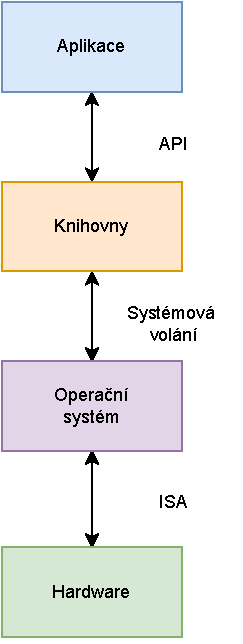
\includegraphics[width=0.325\textwidth]{assets/img/computer_stack.pdf}
    \caption{Architektura počítače ukazující příležitosti k virtualizaci}
    \source{Vytvořeno dle předlohy z \cite{chiueh2005survey}}
    \label{fig:pc_stack}
\end{figure}



\subsection{Možnosti virtualizace}

Jak jsem již nastínil, virtualizační vrstva může existovat na více úrovních. V této sekci bych rád přiblížil virtualizace od nejnižší vrstvy až po tu nejvyšší.

\subsubsection{Virtualizace na úrovni ISA}

ISA, neboli \textit{Instruction Set Architecture} je součástí abstraktního modelu počítače a definuje, jak může software ovládat procesor. ISA funguje jako rozhraní mezi hardwarem a softwarem a specifikuje, co a jak je procesor schopen udělat.\,\cite{isa-arm}

Virtualizace na této úrovni tedy funguje za pomoci softwarové emulace ISA dané platformy. Tedy virtuální vrstva musí být schopna přeložit ISA instrukce hosta na na ISA instrukce hostitele. Tento způsob lze označit i jako \textit{binární překlad}. Tato virtualizace funguje pouze v případě, že existuje způsob, jak na hostitelské platformě provést všechny úkony, požadované architekturou hosta. 

Výhodou této virtualizace je, že nám teoreticky dokáže dát dostatečné prostředky ke spuštění jedné platformy (jako například x86) na ostatních platformách. Taktéž jsme schopni spustit operační systémy, bez žádné modifikace. Tato portabilita ovšem přichází s nemalou cenou. Tím, že musíme každou instrukci softwarově přeložit, tak dochází k velkému snížení výkonu systému. I tak si tento způsob virtualizace nalezne využití. 


\subsubsection{Virtualizace na úrovni HAL}
\customtodo{Vysvětlit co je HAL}

Virtualizace na HAL tedy využívá podobností mezi architekturou platformy hosta a hostitele, díky čemuž může snížit latency způsobenou překladem. Důležitou komponentou v tomto případě je tzv. \textit{hypervizor} (někdy taky označován jako Virtual Machine Monitor - VMM). Hypervizor je softwarová vrstva, která virtualizuje všechny potřebné zdroje fyzického stroje, a tím definuje a podporuje běh jednoho či více VM. \cite{whitaker2002denali}

Existují dva typy hypervizorů. Ty můžeme vidět na obrázku \ref{fig:vm_types}. Hypervizor typu I běží přímo nad hardwarem a spravuje všechny virtuální stroje.

\cite{chiueh2005survey}\cite{RODRIGUEZHARO2012267}

\begin{figure}[htbp]
    \centering 
    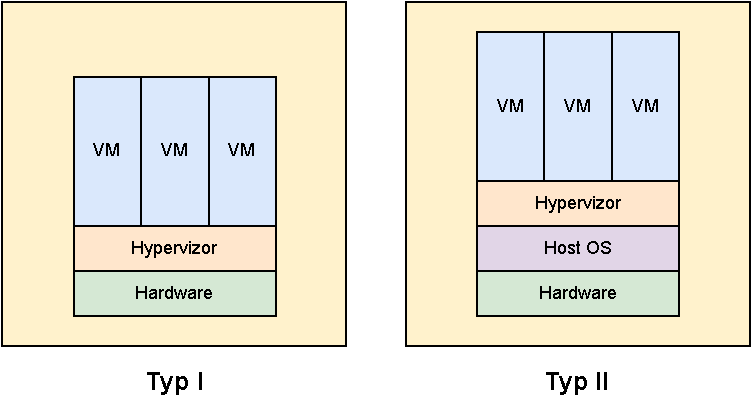
\includegraphics[width=\textwidth]{assets/img/vm_types.pdf}
    \caption{Možné typy virtualizace na úrovni HAL}
    \source{Vytvořeno dle předlohy z \cite{RODRIGUEZHARO2012267}}
    \label{fig:vm_types}
\end{figure}


\subsubsection{Virtualizace na úrovni operačního systému}


\subsubsection{Virtualizace na úrovni programovacího jazyku}


\subsubsection{Virtualizace na úrovni knihoven}

